\documentclass[12pt]{scrartcl}%{article} % Beginn der LaTeX-Datei
%Titel etc

\title{
\begin{flushright}
 
\includegraphics[scale=0.5]{HAW_Marke_RGB_300dpi.jpg}
\end{flushright}

\vspace{2cm}

IT-Systeme\\
Dokumentation
 
\vspace{1cm}

\LARGE Interaktive Videoinstallation mit\\
granularem Synthesizer
}

%\author{}
\date{20. Februar 2024}

% Kopf- und Fußzeilen

\usepackage[headsepline,%footsepline
]{scrlayer-scrpage}
\pagestyle{scrheadings}
\clearpairofpagestyles


\ihead{20.02.2024}
\chead{IT Systeme}
\ohead{Dokumentation: visueller Synthesizer}
\ifoot{}
\cfoot{}
\ofoot{\pagemark}

%% twocolumn

\usepackage{amsmath,amssymb}  % erleichtert Mathe 
\usepackage{enumerate}% schicke Nummerierung

\usepackage{graphicx} % für Grafik-Einbindung
%\usepackage{hyperref}

\usepackage[german]{babel}
\usepackage[T1]{fontenc}
\usepackage{lmodern}
\usepackage{textcomp}
 % Einstellungen, wenn man deutsch schreiben will, z.B. Trennregeln
\usepackage[utf8]{inputenc}  % für Unix-Systeme
  % ermöglicht die direkte Eingabe von Umlauten und ß
  % evt. obige Zeile ersetzen durch
  % \usepackage[ansinew]{inputenc}  % für Windows
  % \usepackage[applemac]{inputenc} % für den Mac


%%%%%%%%%%%%%%%%%%%%%%%%%%%%%%%%%%%%%%%%%%%%%%%%%%%%%%%%%%%%%%%%%%
%
%  ntheorem
%
\usepackage[thmmarks,amsmath,hyperref,noconfig]{ntheorem} 
  % erlaubt es, Sätze, Definitionen etc. einfach durchzunummerieren.
\newtheorem{satz}{Satz}[section] % Nummerierung nach Abschnitten
\newtheorem{hilfssatz}[satz]{Hilfssatz}
\newtheorem{kor}[satz]{Korollar}

\theorembodyfont{\upshape}
\newtheorem{beispiel}[satz]{Beispiel}
\newtheorem{bemerkung}[satz]{Bemerkung}
\newtheorem{definition}[satz]{Definition} %[section]

\theoremstyle{nonumberplain}
\theoremheaderfont{\itshape}
\theorembodyfont{\normalfont}
\theoremseparator{.}
\theoremsymbol{\ensuremath{_\blacksquare}}
\newtheorem{beweis}{Beweis}
\qedsymbol{\ensuremath{_\blacksquare}}
%\theoremclass{LaTeX}
%
% Ende ntheorem
%
%%%%%%%%%%%%%%%%%%%%%%%%%%%%%%%%%%%%%%%%%%%%%%%%%%%%%%%%%%%%%%%%%%


%\pagestyle{empty}
%
% Ändern der bedruckten Fläche der Seite
% \addtolength{\textwidth}{3cm}  % Befehl mit zwei Argumenten
% \addtolength{\textheight}{3cm}
% \hoffset-2cm % verschiebt das Textfenster nach links
% \voffset-5mm % verschiebt das Textfenster nach oben
%
%\parindent=0pt %% keine Einzug zu Beginn von Abs\"atzen
%\parskip=2mm   %% erzeugt einen zusätzliche Zeilenabstand zwischen
                %% Absätzen. Nötig bei \parindent=0pt


%%%%%%%%%%%%%%%%%%%%%%%%%%%%%%%%%%%%%%%%%%%%%%%%%%%%%%%%%%%%%%%%%%
% ermöglicht, farbigen Text zu drucken.
\usepackage{color}
% Und nun werden die Farben definiert - daran können Sie nach Belieben selber rumspielen.
\definecolor{white}{rgb}{1,1,1}
\definecolor{darkred}{rgb}{0.3,0,0}
\definecolor{darkgreen}{rgb}{0,0.3,0}
\definecolor{darkblue}{rgb}{0,0,0.3}
\definecolor{pink}{rgb}{0.78,0.09,0.51}
\definecolor{purple}{rgb}{0.28,0.24,0.55}
\definecolor{orange}{rgb}{1,0.6,0.0}
\definecolor{grey}{rgb}{0.4,0.4,0.4}
\definecolor{aquamarine}{rgb}{0.4,0.8,0.65}

\usepackage[table]{xcolor}% http://ctan.org/pkg/xcolor
\usepackage{lipsum}
\usepackage{wrapfig}



\DeclareMathOperator{\GL}{GL} % einige Macro, siehe am Ende Abschn. 2
\newcommand{\N}{\mathbb{N}}
\newcommand{\Z}{\mathbb{Z}}
\newcommand{\Q}{\mathbb{Q}}
\newcommand{\R}{\mathbb{R}}
\newcommand{\C}{\mathbb{C}}
\newcommand{\cP}{{\mathcal P}} 


\begin{document}

\begin{titlepage}


\maketitle % erzeugt den Kopf


\vfill 

\begin{flushleft}
\begin{tabular}{rlll}
%\cline{1-3}
\textbf{Gruppe:} & Ariane Bachmann & 2552756 & \hspace{5cm} \\
 & Benjamin Ghodsi-Moghaddam & 2582359 & \hspace{5cm} \\
 & Bruno Bühler & 2625322 & \hspace{5cm} \\
  & Dennis Jonca & 2175314 & \hspace{5cm} \\
   & Evan Tanggo Peter Simamora & 2332397 & \hspace{5cm} \\
    & Fabian Brunner &  2600389 & \hspace{5cm} \\
& Rafael Weber & 2623881 & \hspace{5cm} \\\\
%\cline{1-3}
\textbf{Studiengang:} & Meidentechnik B.Sc. WS 23/24 & \hspace{5cm} \\\\
%\cline{1-3}
\textbf{eingereicht bei:} & Malte Sanders & \hspace{5cm} \\ 
%\cline{1-3}
\end{tabular}
\end{flushleft}

\end{titlepage}

\tableofcontents

\newpage

\section{Einleitung}

Im Rahmen des Kurses für IT-Systeme entsteht ein interaktives Projekt. Studierende haben die Möglichkeit, sowohl Hard- als auch Software eigenständig auszuwählen, um ein individuelle Idee zu entwickeln und umzusetzen. Im Folgenden wird das Konzept des ''Visuellen Synthesizers'' präsentiert.

\section{Grundlagen}
\begin{figure}[h]
   \begin{minipage}[b]{.4\linewidth}
      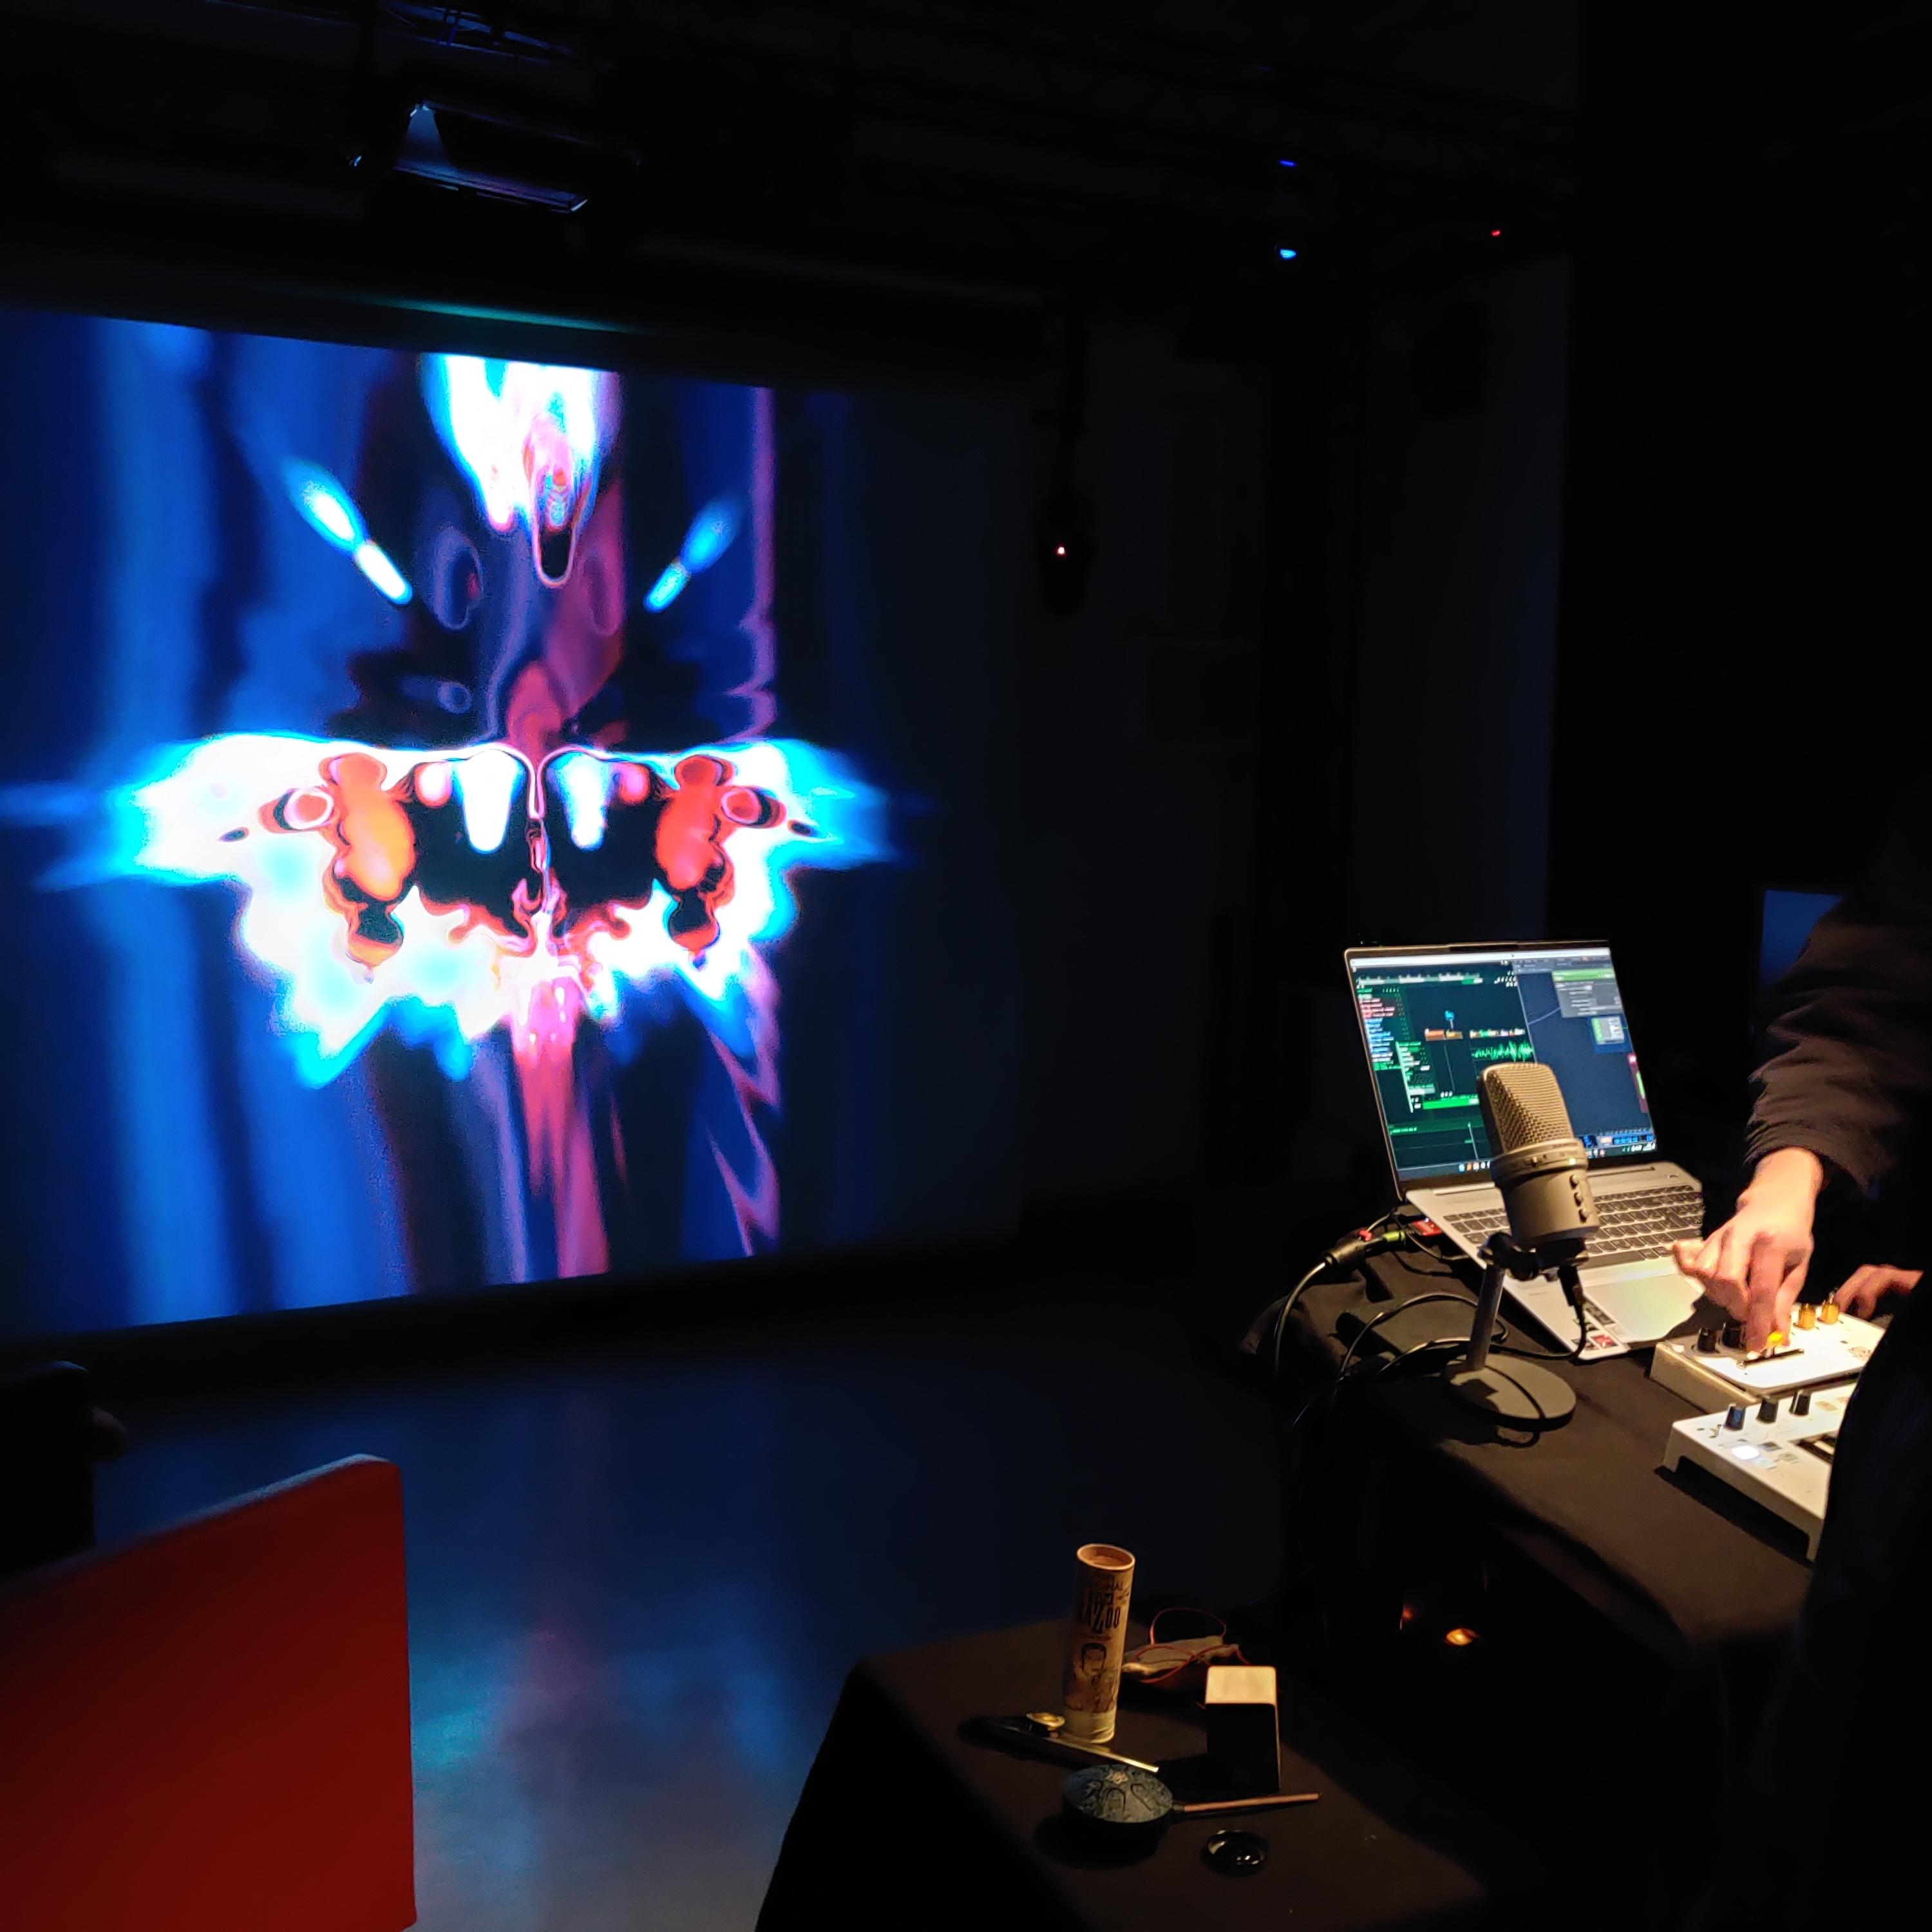
\includegraphics[width=\linewidth]{Rauminstallation}
      \caption{mögliche\\Rauminstallation${}^{1}$}
   \end{minipage}
   \hspace{.1\linewidth}
   \begin{minipage}[b]{.4\linewidth}
      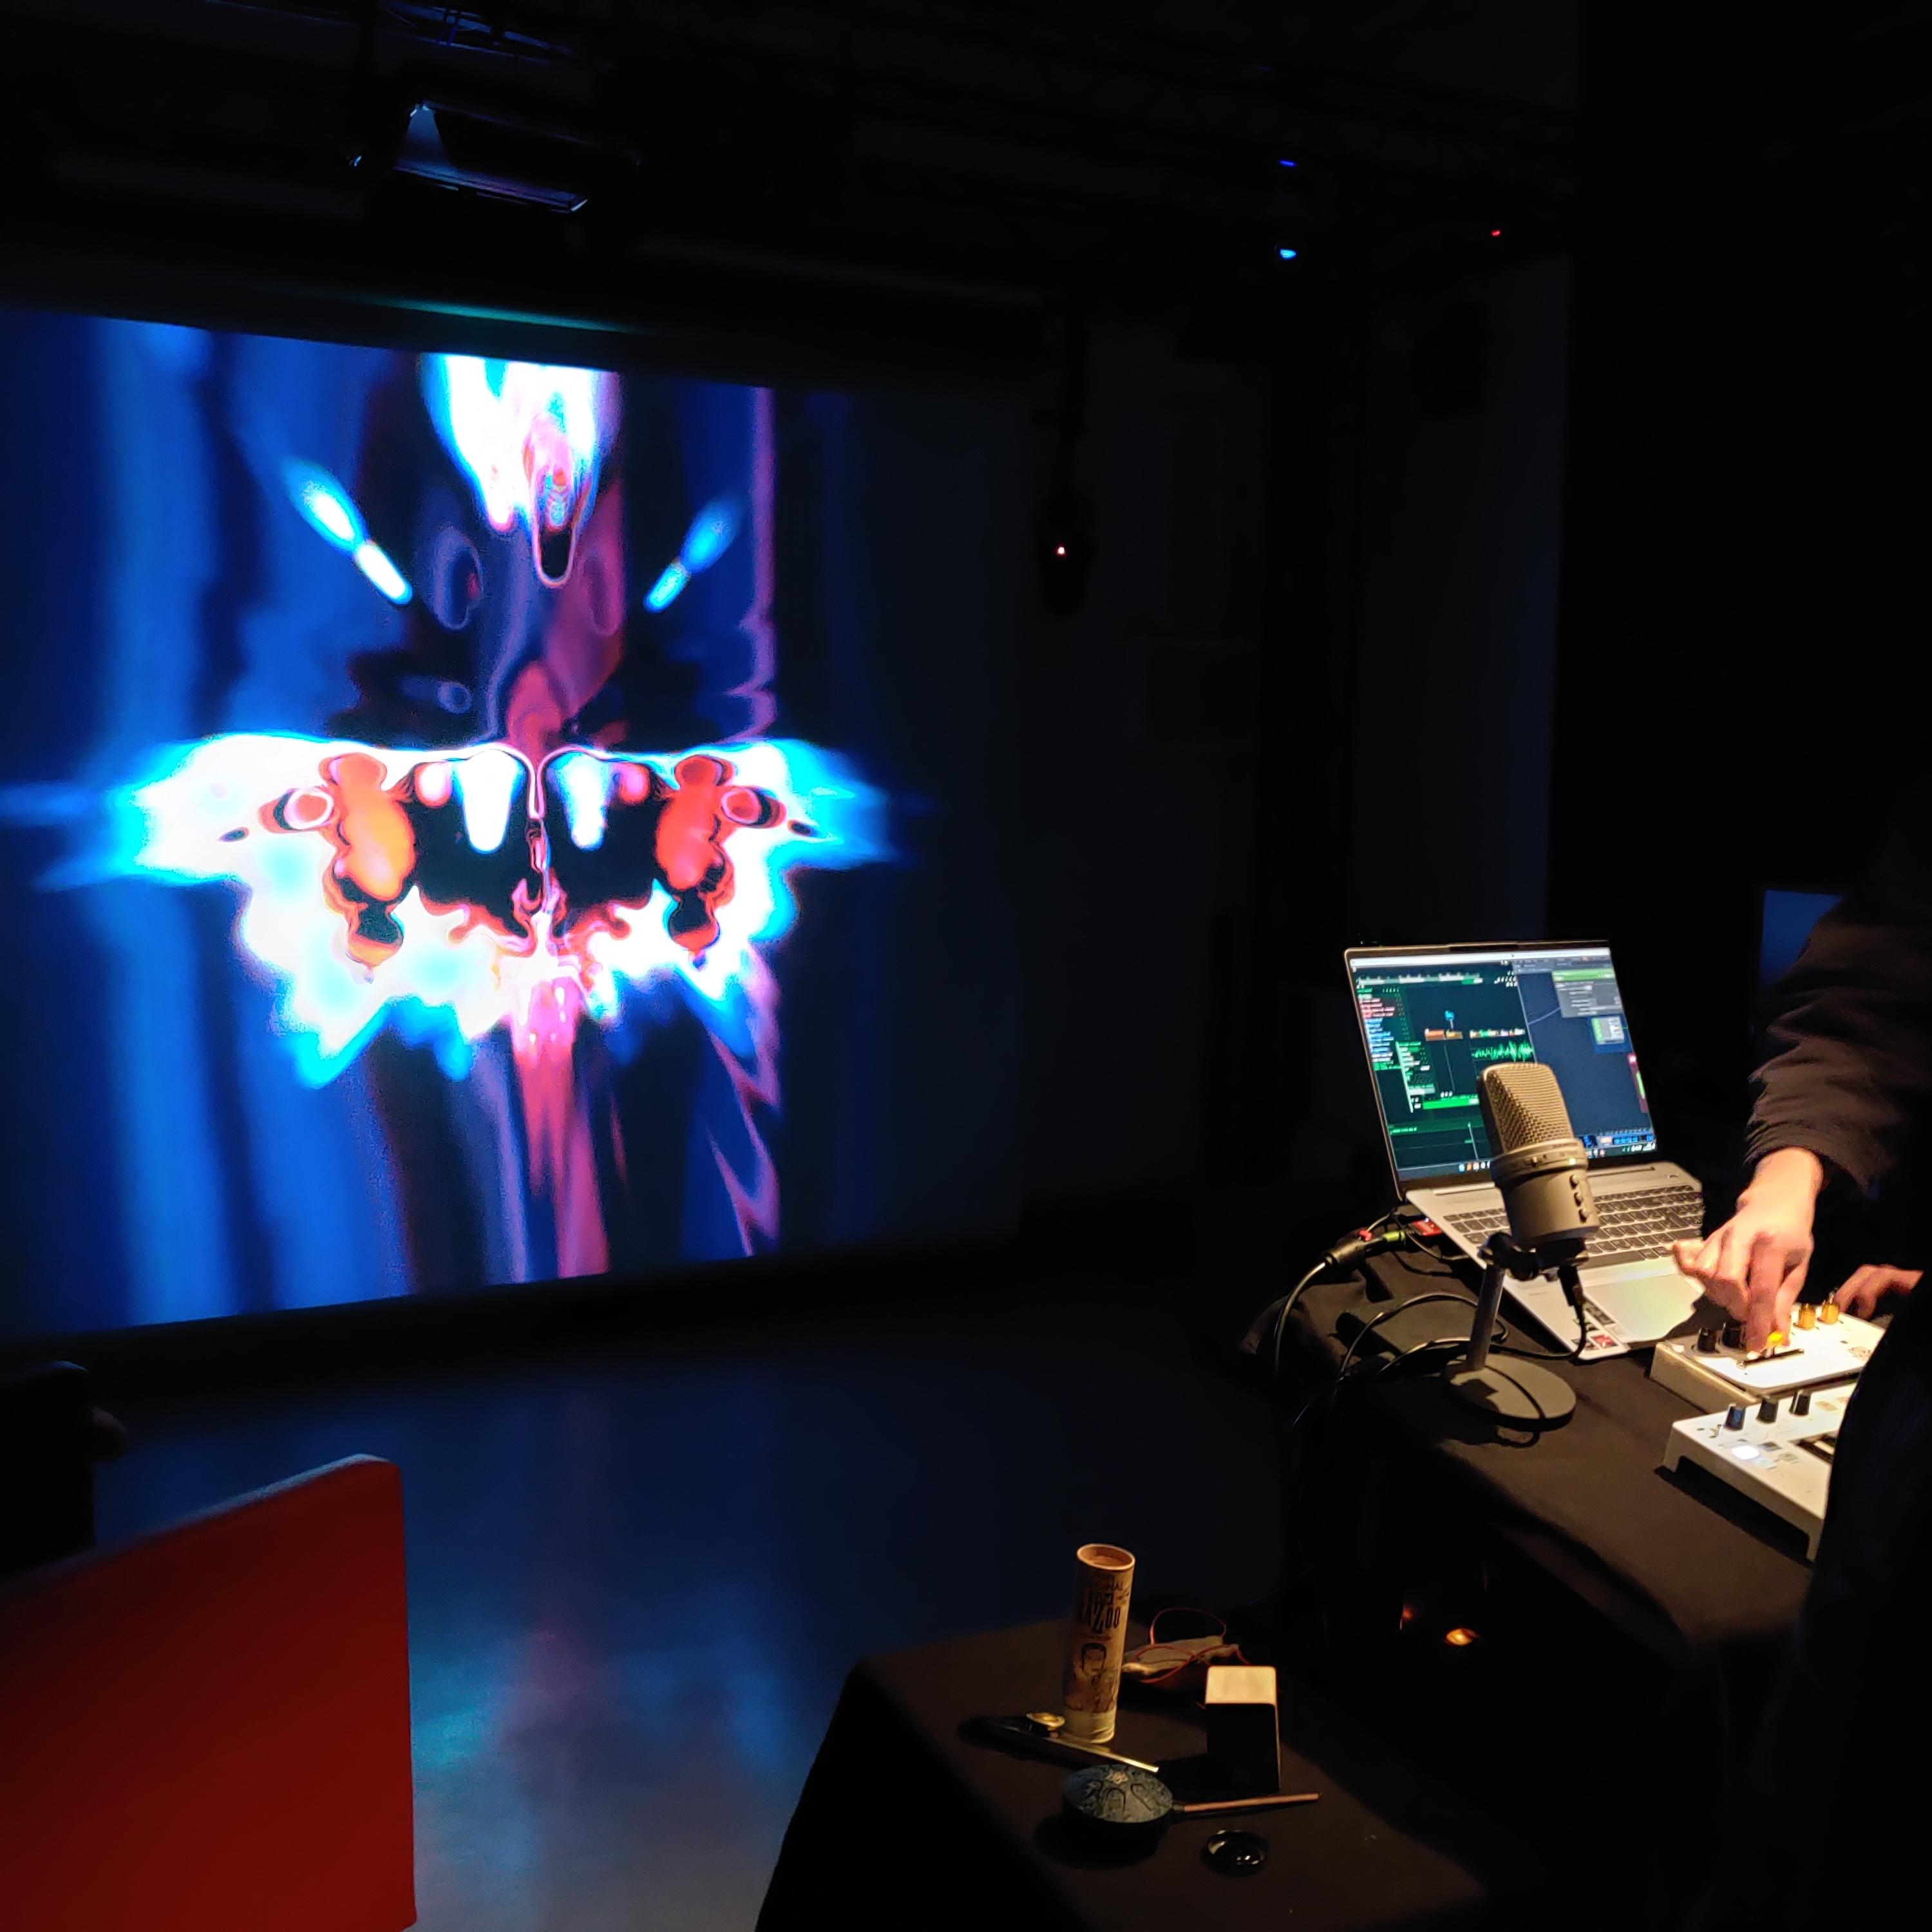
\includegraphics[width=\linewidth]{Rauminstallation}
      \caption{möglicher\\Mikrocontroller${}^{1}$}
   \end{minipage}
\end{figure}
\noindent Die Idee ist, eine Rauminstallation zu entwickeln, die kreativen Ausdruck und Interaktivität verbindet. Im Kern soll ein granularer Synthesizer stehen, der nicht nur außergewöhnliche Klänge erzeugt, sondern auch eine visuelle Dimension hinzufügt. Unabhängig vom Erfahrungsgrad der Nutzenden im Umgang mit Synthesizern und Videoanimation, tauchen diese in eine Welt voller künstlerischer Gestaltung ein. Durch die Kombination von Klangsynthese und visueller Darstellung wird es den Benutzenden ermöglicht, Klänge in Echtzeit zu formen und zu modulieren, während sie gleichzeitig die Wellenformen, Spektren und künstlerischen Visualisierungen dieser Klänge betrachten können.\\\\
Letztendlich soll der gesamte Raum zu einem Instrument verwandelt werden, in dem man isoliert von der Außenwelt eine ganz eigene Atmosphäre schafft und in ständiger Interaktion mit den visuellen und akustischen Eindrücken steht.

\footnotetext[1]{KI generiertes Bild}

\newpage

\section{Konzeption}

Die Besucher betreten einen abgedunkelten Raum, in dessen Mitte sich, beleuchtet von zwei Scheinwerfern, ein Stehtisch befindet, der die notwendigen Bedienelemente beherbergt. Über einen Projektor werden zunächst Standby-Versionen der Visuals an eine Leinwand im vorderen Teil des Raumes projiziert, die später im Einklang mit dem Audio dynamisch verändert werden.
\\\\
Zur Verfügung stehen den Nutzern verschiedene Bedienelemente, darunter ein Mikrofon zur Aufnahme einer Audiospur als Basis für den Granular-Synthesizer, sowie eine kleine Auswahl an Instrumenten und klangbildenden Objekten wie z.B. eine Steel Drum, ein Mini-Cajon, eine Ukulele, ein Kalimba usw. Ein MIDI-Keyboard ermöglicht die Kontrolle der Tonhöhe des Synthesizers. Zusätzlich gibt es einen Mikrocontroller mit sechs Potentiometern zur Steuerung der Synthesizer-Parameter (Frequenz, Spray, Mode, Reverb, Delay, Bitcrush), einem Schieberegler zur Positionierung innerhalb der Audiospur und einem Button zur Steuerung des Visualwechsels.
\\\\

\begin{center}
 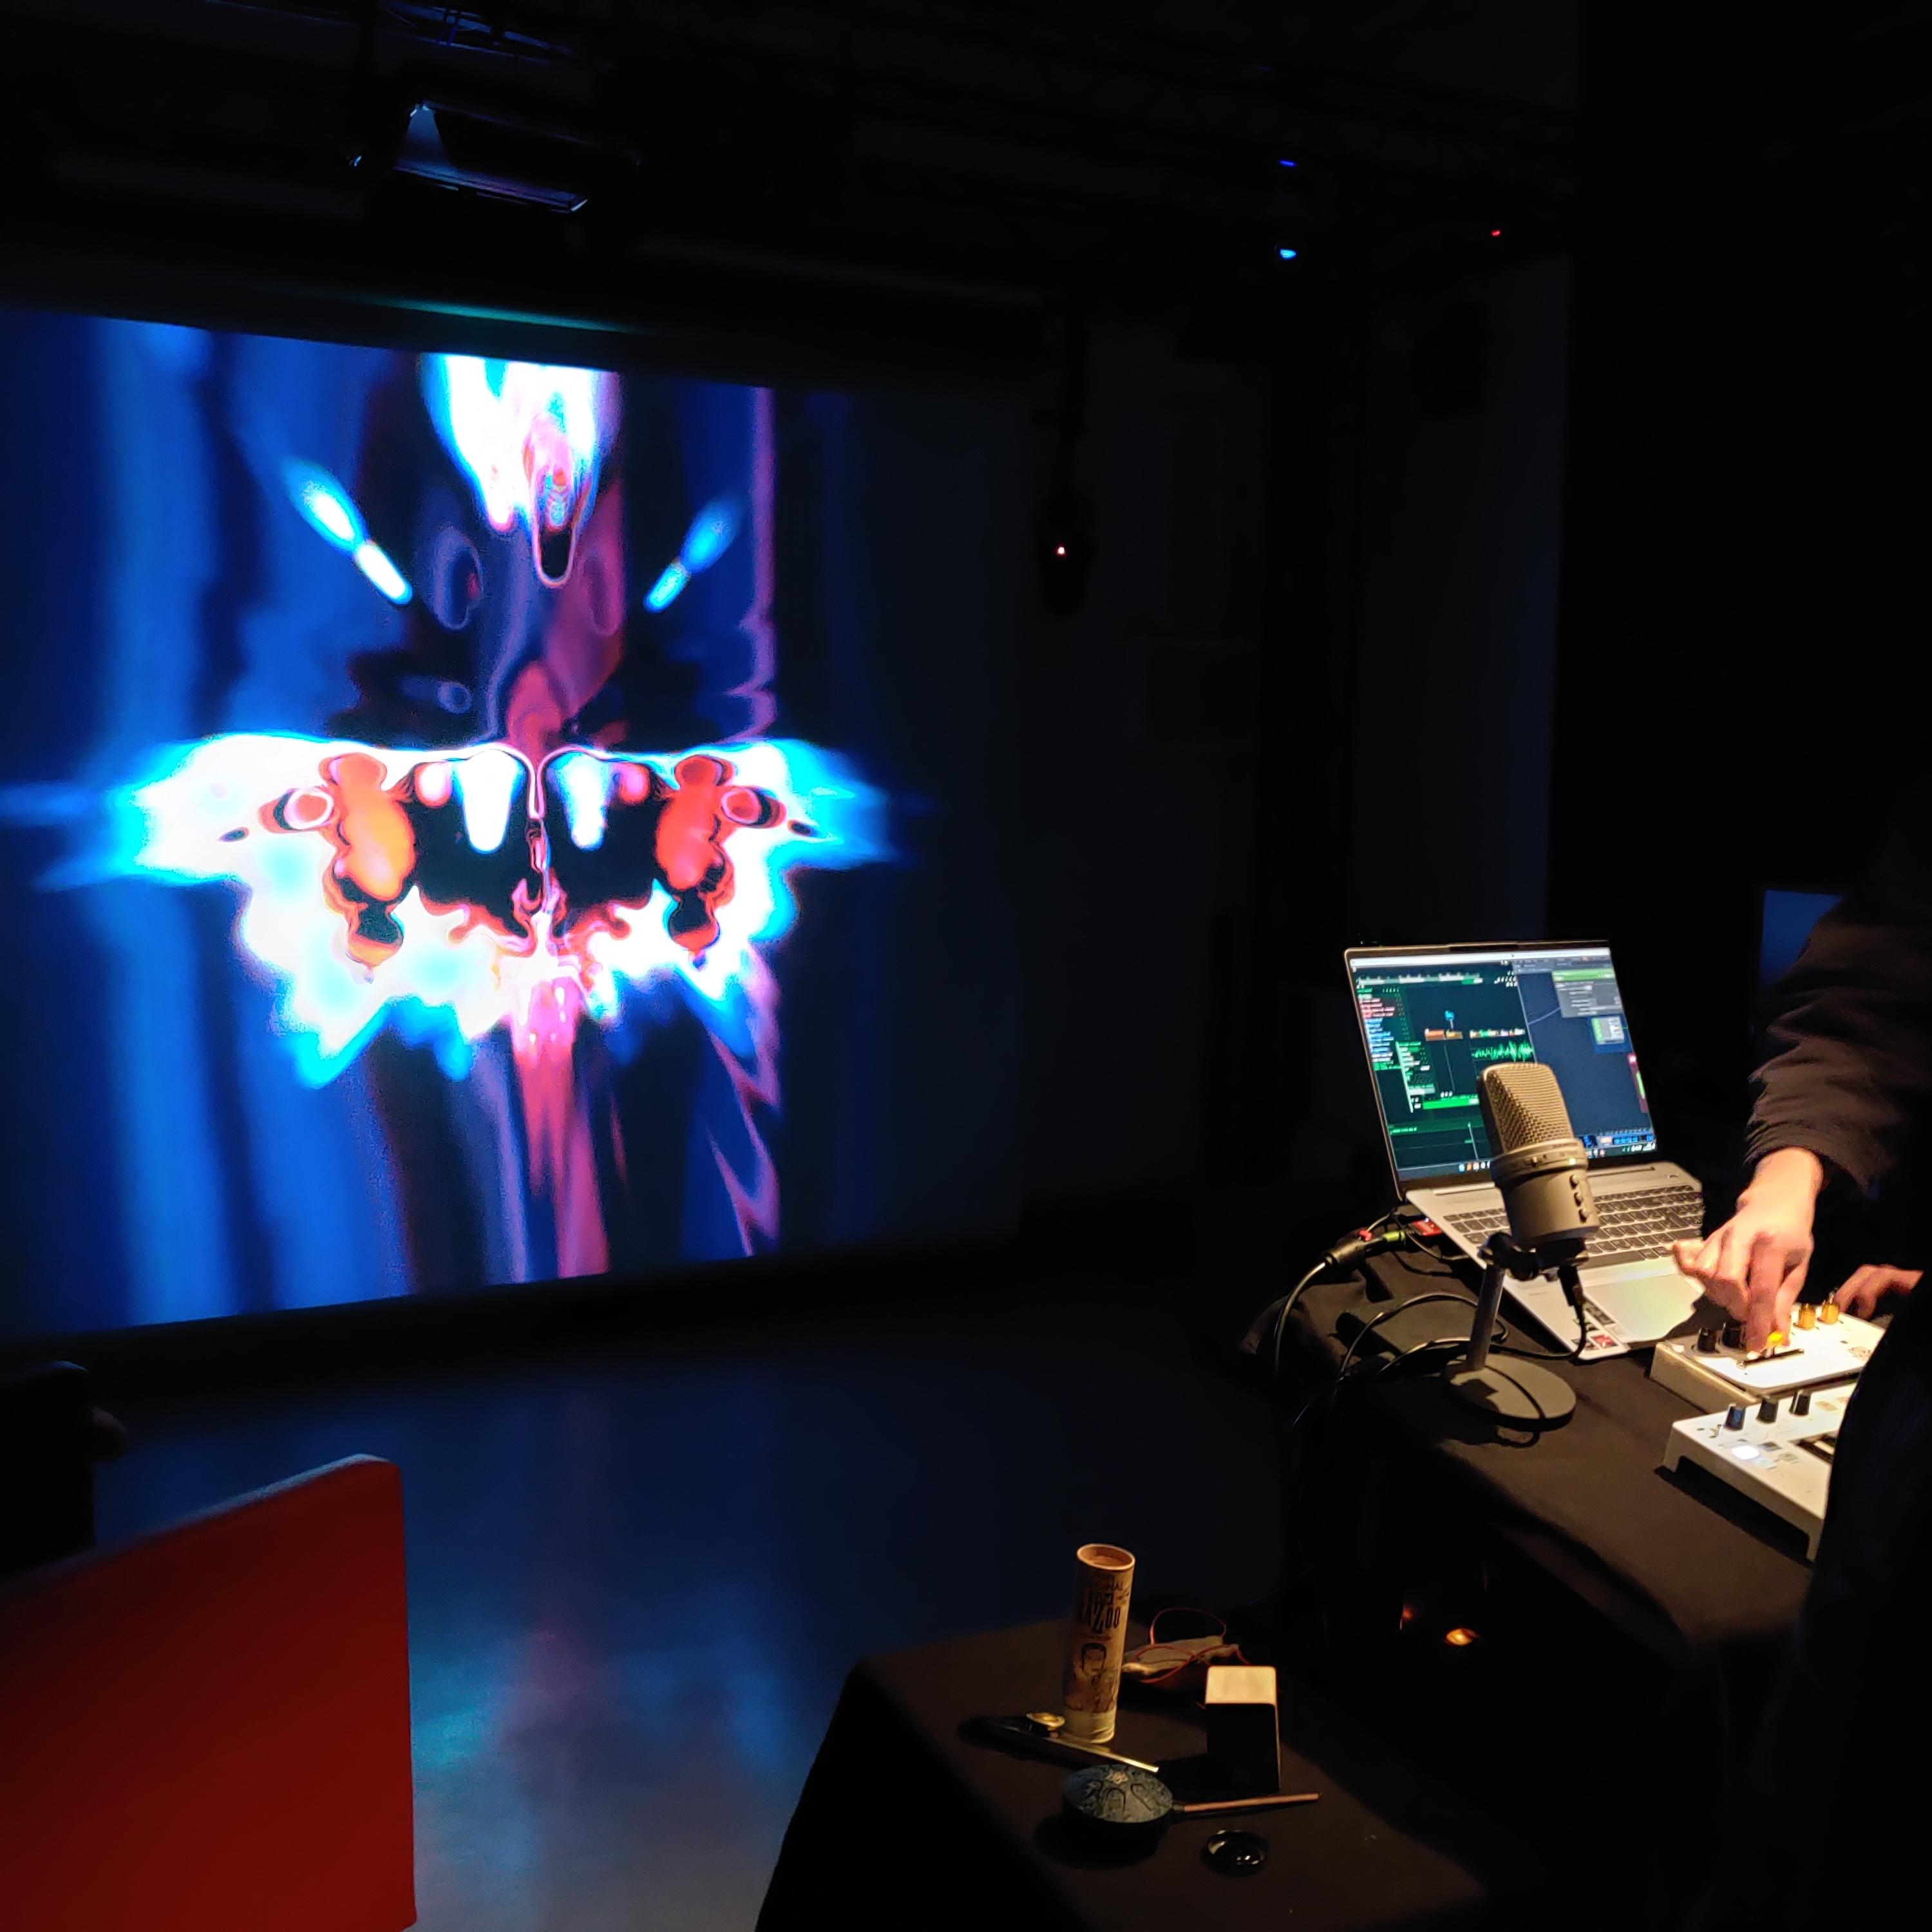
\includegraphics[scale=0.11]{Rauminstallation}
 \captionof{figure}{Rauminstallation}
\end{center}

\newpage

\noindent Der Ablauf beginnt mit der Aufnahme einer Audiodatei über das Mikrofon, indem der Nutzer über den Laptop den Record-Button in der Software SunVox drückt. Nachdem die Aufnahme gestoppt wurde, zeigt der Laptop die Waveform der Audiodatei an. Er ist ab diesem Punkt nur noch Rechenzentrum der Installation, während die Bedienung ausschließlich über das MIDI-Keyboard und den Mikrocontroller erfolgt.
\\\\
Die MIDI-Daten des Mikrocontrollers und des Keyboards werden an den Laptop gesendet, auf dem die Audiosynthese der zuvor aufgenommenen Audiodatei stattfindet. Das resultierende Audiosignal wird über Lautsprecher in den Raum gegeben und gleichzeitig intern an TouchDesigner weitergeleitet. Dort wird das Audiosignal in Echtzeit hinsichtlich seines Frequenzspektrums und seiner Dynamik analysiert und in sechs verschiedene visuelle Darstellungen umgewandelt, die live gerendert und auf eine etwa 2x2m große Leinwand am vorderen Ende des Raumes projiziert werden.
\\\\
Die Visuals wechseln nun automatisch alle zwei Minuten, können aber auch direkt vom Nutzer über einen Button auf dem Mikrocontroller gesteuert werden.
\\\\

\begin{center}
 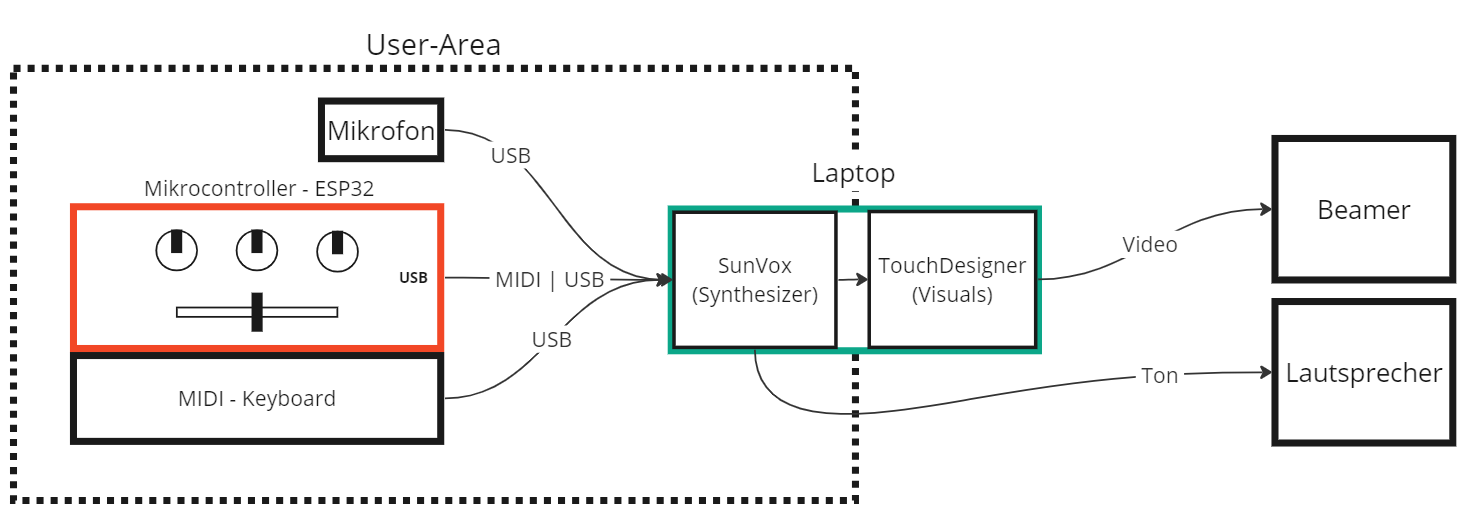
\includegraphics[scale=0.5]{Blockschaltbild}
 \captionof{figure}{Blockschaltbild des kompletten Systems}
\end{center}

\newpage

\section{Projektdurchführung}

\subsection{Zeitplanung}

\subsection{Software}

Nach der Entscheidung, SunVox als Synthesizer Software zu nutzen, galt es zuerst, ein Projekt zu bauen, das die Hauptaspekte der granularen Synthese erfüllt und steuern lässt. Also dass ein Sample zu einem gewählten Punkt in einer bestimmten Frequenz abgespielt werden kann. Das Sample sollte dabei entweder selbst aufgenommen oder ausgewählt werden. Dies ließ sich prinzipiell einfach mit den in SunVox eingebauten Modulen umsetzen.
Es gibt in SunVox das sogenannte MultiSynth Modul, welches allgemein genutzt werden kann, um ein Audiosample abzuspielen und dabei bestimmte Eigenschaften verschiedener Module zu transportieren und auf das jeweilige Sample zu übertragen. Es kann außerdem direkt die angespielte Phase eingestellt werden, weshalb sich darüber endlich auch die Position des Samples bestimmt, die hardwareseitig vom Slider kontrolliert werden sollte. Dass das Sample dann aber nicht nur einmal abgespielt wird, sondern in sich wiederholenden Grains, wird durch einen Low Frequency Oscillator sichergestellt, der auch als Modul in SunVox vorhanden ist. Sobald der MultiSynth gespielt wird, wird auch der LFO angesteuert und triggered in einer einstellbaren Frequenz das Sample immer wieder neu an. Wie lang das Sample abgespielt wird, bestimmt sich im Endeffekt aus der gewählten Frequenz des LFO, um aber darüber hinaus noch mehr vom Sample in einen eingestellten Sound hineinzubekommen, lässt sich die gewählte Position, die Phase des MultiSynth, auch mehr oder weniger randomisieren, was zu einer Art Position Spray führt, was noch mehr Abwechslung in die Soundgestaltung bringen sollte.
Ein großer Pluspunkt für SunVox ist die einfache Anbindung von MIDI-Geräten. Ein jeweiliger Controller muss nur am Rechner angeschlossen sein und man kann Parameter für Parameter auf die Bedienelemente legen wie man will. Dabei hätte man sogar experimentell mehrere Parameter auf ein Potentiometer mappen können. Für das MIDI-Keyboard, das zum Spielen verwendet werden sollte, musste nur festgelegt werden, welches Modul die Keyboard-MIDI-Befehle annehmen soll. Das war entsprechend unser selbst gebautes Granulator Modul.
Das Sampler Modul von SunVox stellt exakt die gewünschten Funktionen zum Aufnehmen und Reinladen von Samples bereit. Problem hier war aber, dass diese Funktionen nur per Mausklick im Interface auswählbar sind, was die Vorstellung einer vollends über Bedienelemente am Mikrocontroller gesteuerten Installation störte. Eventuell wäre es möglich gewesen, wenn man, statt direkt mit der SunVox Software zu arbeiten, die ebenso vorhandene Library genutzt hätte, die sich über Code steuern lässt. Die Entscheidung fiel dann aber schnell darauf, mit dem Programm weiterzuarbeiten und lieber die Installation anzupassen und flexibler zu gestalten, da es einerseits übersichtlicher ist und grade im Zusammenspiel mit der Peripherie um einiges schneller und flexibler in Sachen Konfiguration und Fehleranalyse ist und es andererseits deutlich mehr Zeit benötigt hätte, sich da hineinzuarbeiten, um am Ende eventuell festzustellen, dass die Installation aus welchen Gründen auch immer trotzdem nicht wie geplant umgesetzt werden kann. Zudem bietet SunVox mit dem Sampler die Möglichkeit, die Waveform des Samples anzeigen zu lassen, inklusive Cursor, der anzeigt, wo das Sample aktuell abgespielt wird. Eine solche Visualisierung war von Anfang an für die Installation vorgesehen, nur war nicht eindeutig, wie sie eingebunden werden kann. So fiel dann die Entscheidung, einen extra Bildschirm respektive den Laptop, über den die Software am Ende lief, aufzustellen, um die Steuerung und damit die Funktionalität der Installation sicher zu stellen und gleichzeitig noch die Waveform anzeigen zu können.
\\\\
Somit stand schnell ein Projekt, dass grundlegend als Granular Synthesizer funktioniert. Von da an war die Hauptaufgabe, auszuloten, welche ansteuerbaren Parameter sich in SunVox am besten für die Bedienung an unserer Hardware eignen. Viele Optionen standen zur Auswahl, die teilweise stark den Sound beeinflussten, wie zum Beispiel die Randomisierung der Tonhöhe. Um es nicht zu kompliziert zu halten, da es ohnehin mit einem gewissen Anspruch verbunden ist, den Synthesizer zu spielen, wurden am Ende aber nur die wichtigsten Parameter Position, Loop Frequency, Position Spray sowie die, die den Sound nochmal abrunden, Reverb, Delay und Distortion gemappt (letztere waren ebenfalls direkt als Modul in SunVox vorhanden).
\\\\
Um zusätzlich das Problem zu beheben, dass es zu Artefakten in der Audio kommt, wenn das Sample durch die gewählte Position bei hoher Amplitude abgehakt wird, wurde noch versucht, mit einem ADSR Attack und Release für die Grains einstellbar zu machen, allerdings hat dieser nicht wie erwartet für die einzelnen Grains gegriffen, sondern nur für einen gespielten Input, der natürlich viele Grains hintereinander triggered. Als Alternative lässt sich die Hüllkurve des Samples zwar direkt im Sampler selbst einstellen, dies muss aber jedes Mal aufs Neue manuell gemacht werden, sobald ein neues Sample geladen wird. Das wurde dann aber entsprechend in Kauf genommen und es blieb bei den genannten Parametern, die die Hardware steuern sollte.

\newpage


\subsection{Hardware}

\newpage

\subsection{Touch Designer}

In Touch-Designer wollten wir interessante, audioreaktive Visuals erzeugen, die den granularen Synthesizer visuell untermahlen. Wir haben außerdem den Anspruch gehabt, dass zwischen den Visuals automatisch umgeschaltet wird und auch manuelles Umschalten möglich machen.
\\\\
\textbf{Gesamtstruktur}
\\\\
In der Gesamtstruktur des Touch-Designer Files sind die einzelnen Visuals als .tox Dateien eingefügt. Auf diese Weise können alle Visuals parallel laufen. Am Anfang gibt es einen Audioinput, auf den Alles Visuals zugreifen. So wird nicht für jedes Visual ein eigener Input benötigt, sondern alle haben nur einen „In“ Chop, über den alle auf den gleichen Audioinput zugreifen können. Am Ende jeder .tox Datei ist ein „Out“ Chop, worüber die Ausgänge der Visuals alle in einen „Switch“ laufen. Dieser Switch geht in ein „Cross“. In den anderen Eingang des „Cross“ geht ein schwarzes Bild, welches für den Übergang zwischen den Visuals benötigt wird. Am Ausgang des „Cross“ hängt ein „Window“, welches der finale Ausgang für Touch-Designer ist. Für den Übergang gibt es einen automatischen und einen manuellen Modus. Im Automatischen Modus zählt ein Timer hoch, der nach einer bestimmten Zeit den Übergang auslöst. Beim Übergang wechselt der „Cross“ für einen kurzen Moment auf das schwarze Bild. Hier gibt es einen Fade und keinen harten Cut. In dem Moment, indem das Bild Vollständig schwarz wird, springt der „Switch“ auf das nächste Visual und der „Cross“ fadet aus dem schwarzen Bild zurück auf das neue Visual. Für den manuellen Modus gibt es einen extra Knopf auf dem Controller, der ein Midi Signal an Touch-Designer schickt und den Übergang einleitet. Nach dem manuellen Wechsel bleibt das ausgewählte Visual für eine bestimmte Zeit stehen. Läuft diese Zeit ab, ohne dass der Knopf erneut gedrückt wurde, springt Touch-Designer wieder in den automatischen Modus, damit nicht dauerhaft ein Visual stehen bleibt, sobald der Knopf einmal gedrückt wurde. 

\begin{center}
 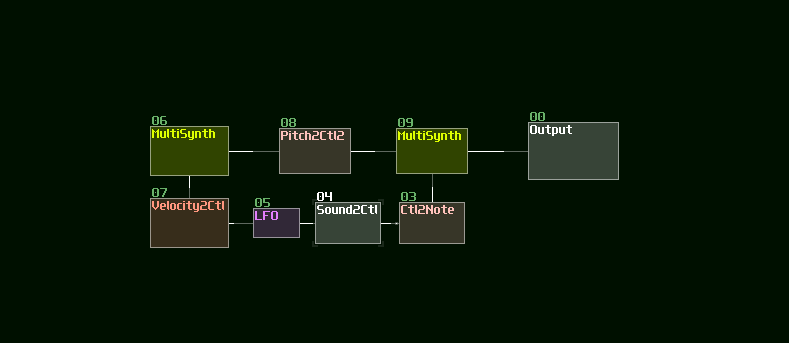
\includegraphics[scale=0.9]{sunvox_1}
 \captionof{figure}{SSS}
\end{center}

\newpage

\noindent \textbf{Visuals}
\begin{figure}[h]
   \begin{minipage}[b]{.4\linewidth}
     ,,Color Blobs'':
     \\\\
In diesem Audio-Visualizer wird das Spektrum des Audio-Inputs genutzt, um Kreise zu erstellen und deren Größe zu verändern. Diese werden durch eine Aneinanderreihung von Feedback, Blur, Displace, Mirror und anderen TOP-Nodes zu einem Interessanten, sich bewegenden „rohrschachtest-artigen“ Muster. Die Farbgebung wird über eine Ramp- und einen Lookup-TOP gesteuert.
   \end{minipage}
   \hspace{.1\linewidth}
   \begin{minipage}[b]{.4\linewidth}
      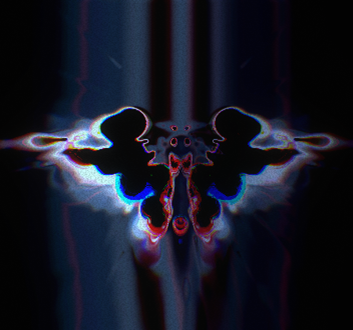
\includegraphics[width=\linewidth]{sunvox_2}
      \caption{möglicher\\Mikrocontroller${}^{1}$}
   \end{minipage}
\end{figure}
\begin{figure}[h]
   \begin{minipage}[b]{.4\linewidth}
     „Point Cloud“:
     \\\\
     Eine Röhre wird verformt und durch ein Noise-TOP geschickt, das Abbild der Röhre wird dann durch 	eine Point Cloud aus kleinen Quadraten abgebildet. Das Noise wird durch den Audio-Input verändert, 	was die Audio-Reaktivität erzeugt.
   \end{minipage}
   \hspace{.1\linewidth}
   \begin{minipage}[b]{.4\linewidth}
   \vspace{50pt}
      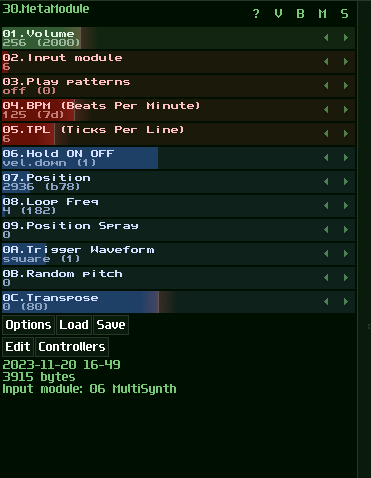
\includegraphics[scale=1]{sunvox_3}
      \caption{möglicher\\Mikrocontroller${}^{1}$}
   \end{minipage}
\end{figure}
\begin{figure}[h]
   \begin{minipage}[b]{.4\linewidth}
     ,,Color Blobs'':
     \\\\
In diesem Audio-Visualizer wird das Spektrum des Audio-Inputs genutzt, um Kreise zu erstellen und deren Größe zu verändern. Diese werden durch eine Aneinanderreihung von Feedback, Blur, Displace, Mirror und anderen TOP-Nodes zu einem Interessanten, sich bewegenden „rohrschachtest-artigen“ Muster. Die Farbgebung wird über eine Ramp- und einen Lookup-TOP gesteuert.
   \end{minipage}
   \hspace{.1\linewidth}
   \begin{minipage}[b]{.4\linewidth}
      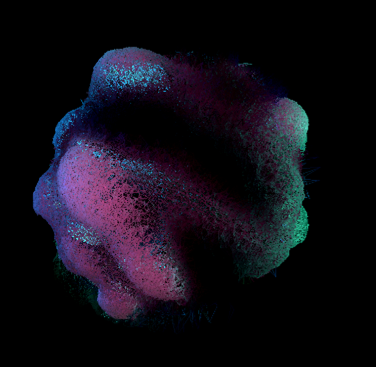
\includegraphics[width=\linewidth]{sunvox_4}
      \caption{möglicher\\Mikrocontroller${}^{1}$}
   \end{minipage}
\end{figure}
\begin{figure}[h]
   \begin{minipage}[b]{.4\linewidth}
     ,,Color Blobs'':
     \\\\
In diesem Audio-Visualizer wird das Spektrum des Audio-Inputs genutzt, um Kreise zu erstellen und deren Größe zu verändern. Diese werden durch eine Aneinanderreihung von Feedback, Blur, Displace, Mirror und anderen TOP-Nodes zu einem Interessanten, sich bewegenden „rohrschachtest-artigen“ Muster. Die Farbgebung wird über eine Ramp- und einen Lookup-TOP gesteuert.
   \end{minipage}
   \hspace{.1\linewidth}
   \begin{minipage}[b]{.4\linewidth}
      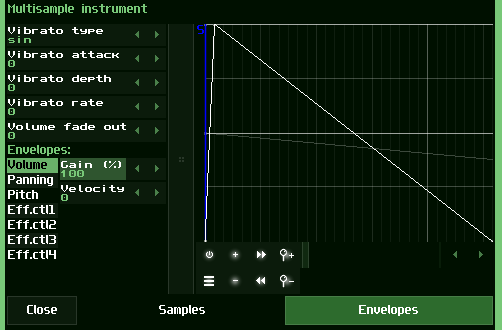
\includegraphics[width=\linewidth]{sunvox_5}
      \caption{möglicher\\Mikrocontroller${}^{1}$}
   \end{minipage}
\end{figure}
\begin{figure}[h]
   \begin{minipage}[b]{.4\linewidth}
     ,,Color Blobs'':
     \\\\
In diesem Audio-Visualizer wird das Spektrum des Audio-Inputs genutzt, um Kreise zu erstellen und deren Größe zu verändern. Diese werden durch eine Aneinanderreihung von Feedback, Blur, Displace, Mirror und anderen TOP-Nodes zu einem Interessanten, sich bewegenden „rohrschachtest-artigen“ Muster. Die Farbgebung wird über eine Ramp- und einen Lookup-TOP gesteuert.
   \end{minipage}
   \hspace{.1\linewidth}
   \begin{minipage}[b]{.4\linewidth}
      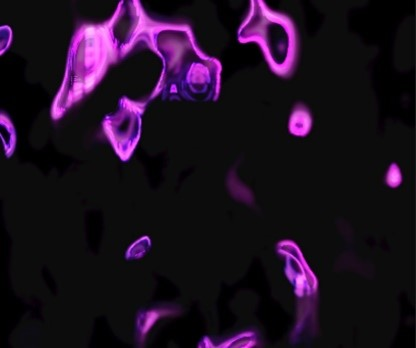
\includegraphics[width=\linewidth]{sunvox_6}
      \caption{möglicher\\Mikrocontroller${}^{1}$}
   \end{minipage}
\end{figure}


\newpage

\section{Fazit}

\subsection{Zusammenfassung}

Zu SunVox lässt sich insgesamt sagen, dass es für Audiosynthese und elektronische Musik für ein kostenloses Programm ein mächtiges Werkzeug ist. Leider ist es eher darauf programmiert, Songs zu gestalten und zu produzieren und weniger, selbst als Instrument genutzt zu werden. Das führte eben dazu, dass in der Ausgestaltung der Installation einige Kompromisse gefällt werden mussten, da einfache Funktionen wie ein Shortcut zur Aufnahme von Samples in der Software nicht vorhanden sind. Jedoch lässt sich, was den Synthesizer angeht, ein positives Bild ziehen. Trotz der teilweise umständlichen Steuerung von SunVox ist das Ergebnis ein guter Granular Synthesizer, der sich kreativ spielen lässt und mit den Visuals aus TouchDesigner harmoniert.

\subsection{Ausblick}

\subsection{Hardware}

\subsection{Touch Designer}

\section{Systembeschreibung}

Die Systembeschreibung dient der Konkretisierung der Use-Cases sowie ihrer Umsetzung. Dabei werden die Anforderungen mithilfe der MoSCoW-Methode erläutert und die Komponenten der Umsetzung durch ein Systemabbild dargestellt.

\subsection{MoSCoW Priorisierung}

Die Hauptpriorität des Projekts liegt in der Erfüllung der Produktvision, die darauf abzielt, Audio und Video interaktiv zu gestalten. Während zahlreiche weitere Funktionen wünschenswert oder teilweise optional sind, ist es entscheidend, das Produkt so zugänglich wie möglich für Personen zu gestalten, die keine Erfahrung mit Synthesizern oder Videoanimation haben. Die Bedienung soll intuitiv und benutzerfreundlich gestaltet sein.
\begin{enumerate}[]
\item \textbf{Must}
  \begin{enumerate}[-]
  \item Die Synthese der Audiospur wird verarbeitet.
  \item Audiospur wird interaktiv durch die Nutzenden verändert.
  \item Die Interaktion wird durch digitale Visualisierungen dargestellt.
  \end{enumerate}
\item \textbf{Should}
  \begin{enumerate}[-]
  \item Die Aufnahme am Mikrofon wird zur Verarbeitung gespeichert.
  \item granulare Synthese mit den Parametern Grain Pitch, Grain Speed, Grain Scan und Reverb.
  \item Visualisierungen werden durch TouchDesigner entwickelt und wiedergegeben.
  \end{enumerate}
\item \textbf{Could}
  \begin{enumerate}[-]
  \item Die Aufnahme am Mikrofon wird in Echtzeit verarbeitet.
  \item Die entstandene Waveform der Audiospur kann für die Nutzenden angezeigt werden.
  \item Der Audio-Pitch kann an einem MIDI-Keyboard gesteuert werden.
  \item Es gibt mehrere Designs durch TouchDesigner.
  \item Die Nutzenden können aus mehreren Designs selbst wählen.
  \end{enumerate}
\item \textbf{Won't}
  \begin{enumerate}[-]
  \item zu viele Ablenkungen des Users (zweite GUI, etc.).
  \item zu komplexe Bedienung des Controllers für die Nutzenden.
  \end{enumerate}
\end{enumerate}

\subsection{Der Systemaufbau}

Die Nutzenden haben verschiedene Bedienungsmöglichkeiten zur Verfügung. Dazu gehören ein Mikrofon, dessen Aufnahmen als Grundlage für den Granular-Synthesizer dienen, Knöpfe zum Starten und Stoppen der Mikrofonaufnahme, Potentiometer und Slider, die die Steuerung der Synthesizer-Parameter ermöglichen, sowie ein MIDI-Keyboard zur Tonhöhenkontrolle des Synthesizers.\\\\
Zusätzlich könnte es eine Anzeige der aufgenommenen Audiospur in Form einer Waveform geben. Der Mikrocontroller und das Keyboard senden MIDI-Daten an einen Computer, auf dem die Audiosynthese der zuvor aufgenommenen Audiodatei stattfindet. Das resultierende Audiosignal wird zum einen über Lautsprecher im Raum wiedergegeben und zum anderen zusammen mit den MIDI-Daten an TouchDesigner weitergeleitet. Sowohl Audio als auch MIDI beeinflussen die Visualisierung, die über einen Beamer mittels HDMI in den Raum projiziert wird.
\begin{center}
 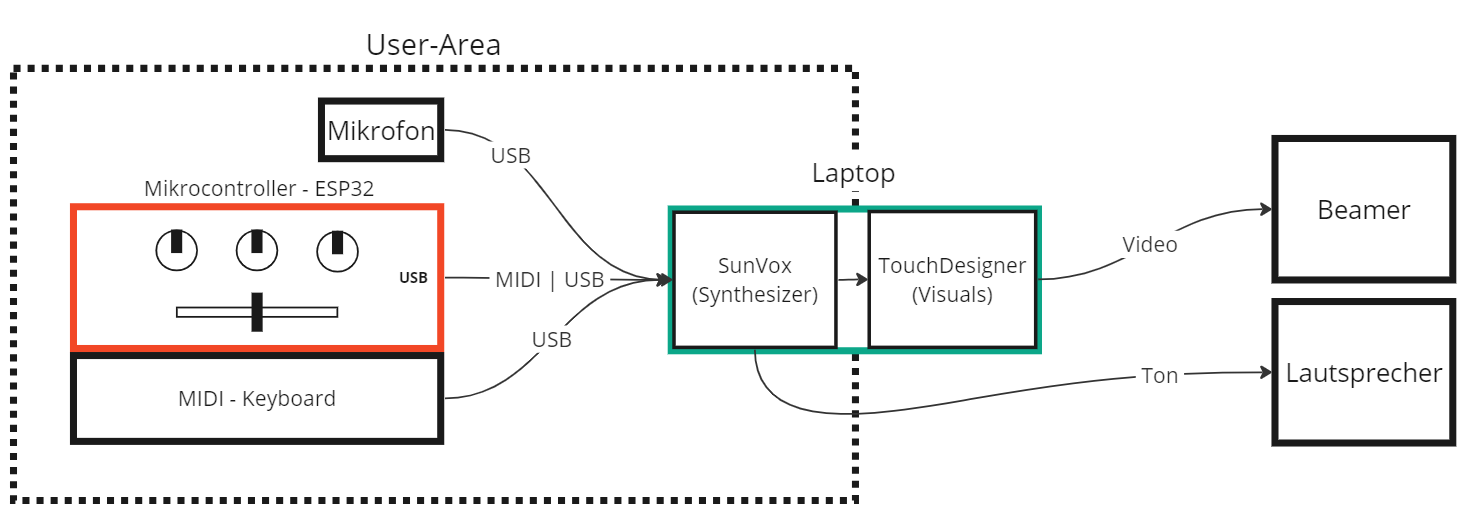
\includegraphics[scale=0.43]{Blockschaltbild}
 \captionof{figure}{Blockschaltbild des kompletten Systems${}^{2}$}
\end{center}

\footnotetext[2]{Miro Board Grafik}

\newpage
\subsection{Use Cases}
Die Use Cases sind im folgenden Szenario beschrieben:\\
Eine Person tritt an die Installation heran und beginnt, Klänge durch die Verwendung des Mikrofons aufzunehmen. Mit den Poti's und Schiebereglern steuert die Person die Klang- und visuellen Effekte. Durch das MIDI-Keyboard werden die Töne gesteuert. Die aufgenommenen Audiospuren und manipulierten visuellen Effekte werden in Echtzeit wiedergegeben, sodass die Nutzenden eine unmittelbare kreative Interaktion erleben.
\begin{center}
 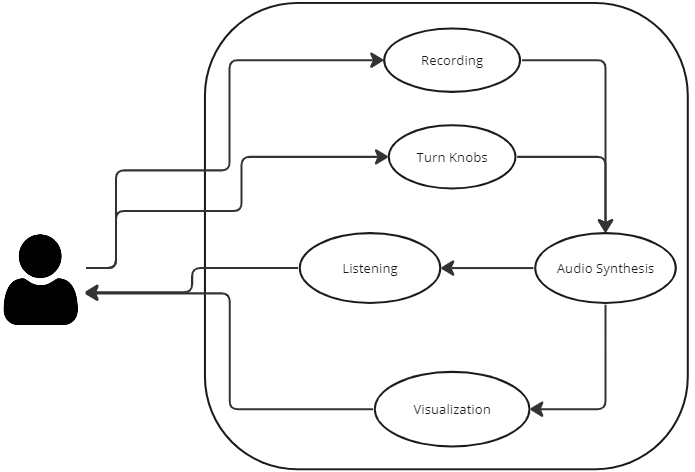
\includegraphics[scale=0.4]{usecases2.png}
 \captionof{figure}{Usecase Diagramm des Projekts${}^{3}$}
\end{center}
\footnotetext[3]{Miro Board Grafik}
\newpage
\section{Roadmap}
Die Roadmap bietet einen zeitlichen Rahmen für das Projekt. Sie enthält alle Projektwochen und einen konzipierten Ablaufplan. Dieser kann sich gemäß den Prinzipien des agilen Projektmanagements während des Projekts verändern.
\begin{flushleft}
 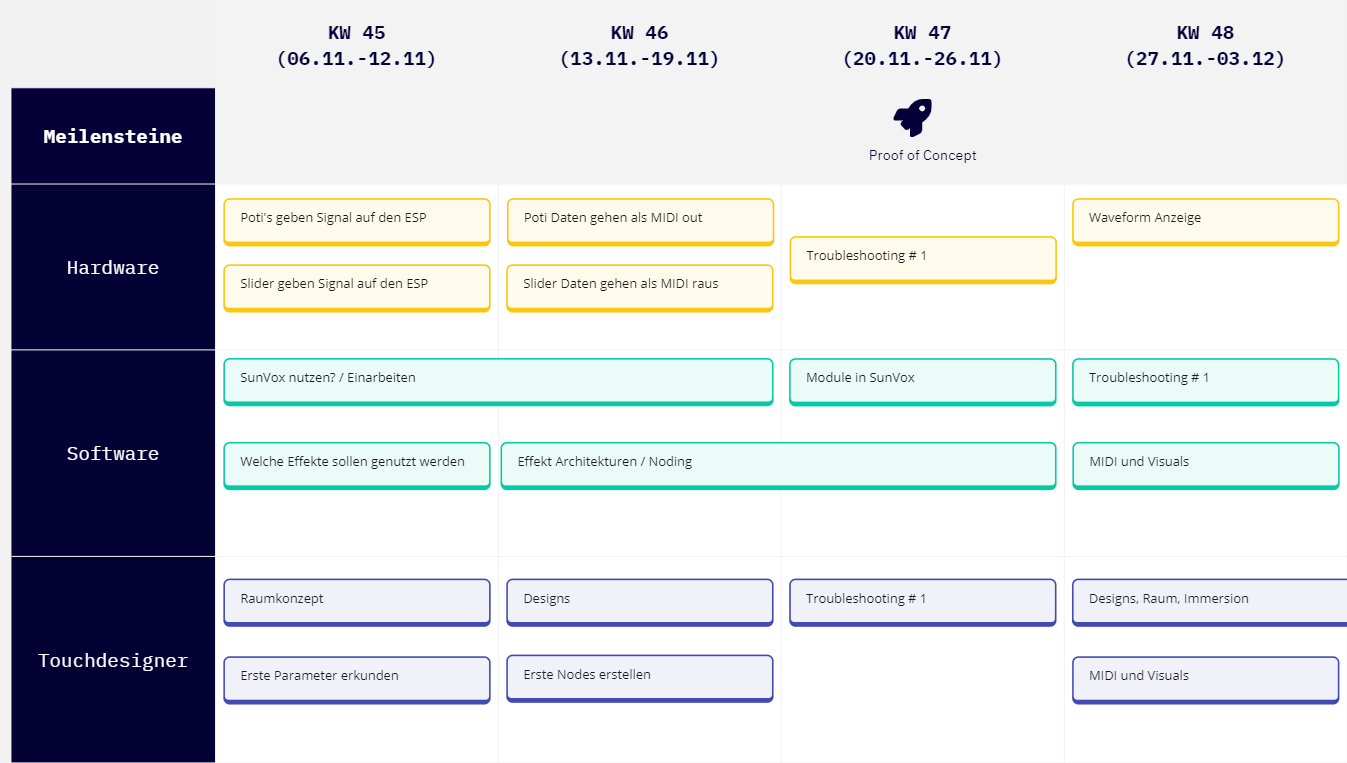
\includegraphics[scale=0.4]{road1.png}
 \captionof{figure}{Roadmap Teil 1${}^{4}$}
\end{flushleft}
\footnotetext[4]{Miro Board Grafik}
\begin{flushleft}
 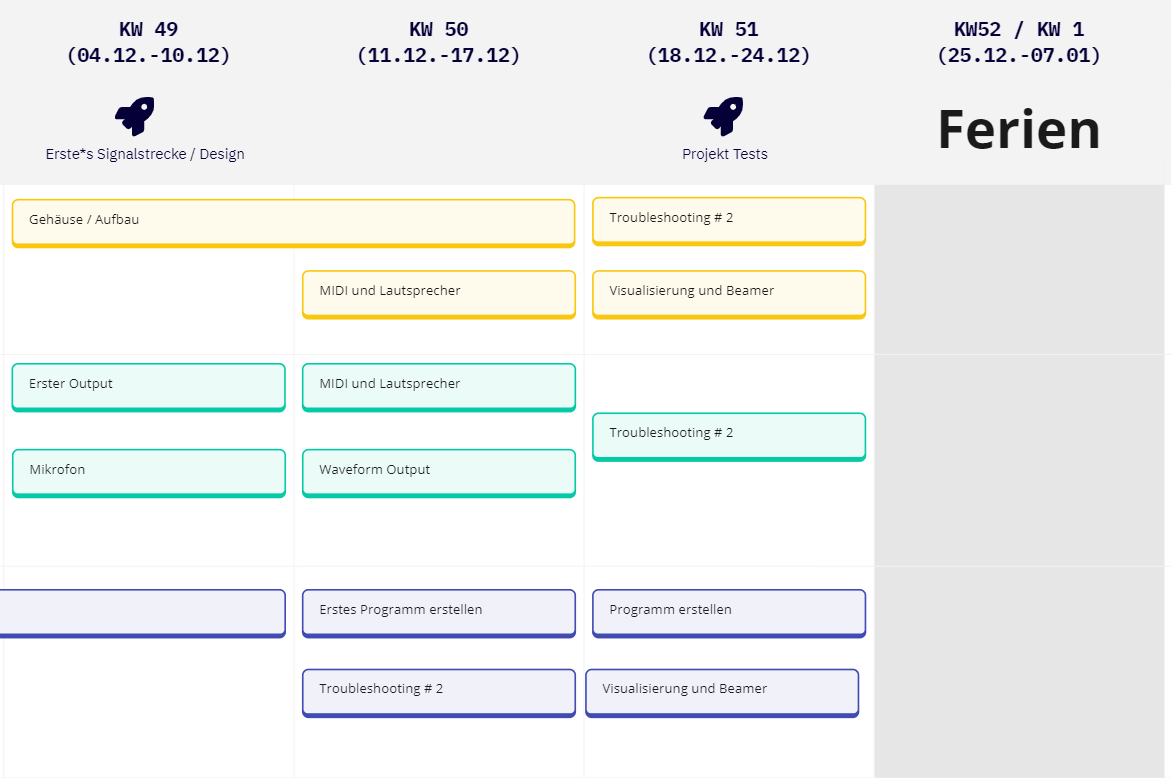
\includegraphics[scale=0.4]{road2.png}
 \captionof{figure}{Roadmap Teil 2}
\end{flushleft}
\begin{flushleft}
 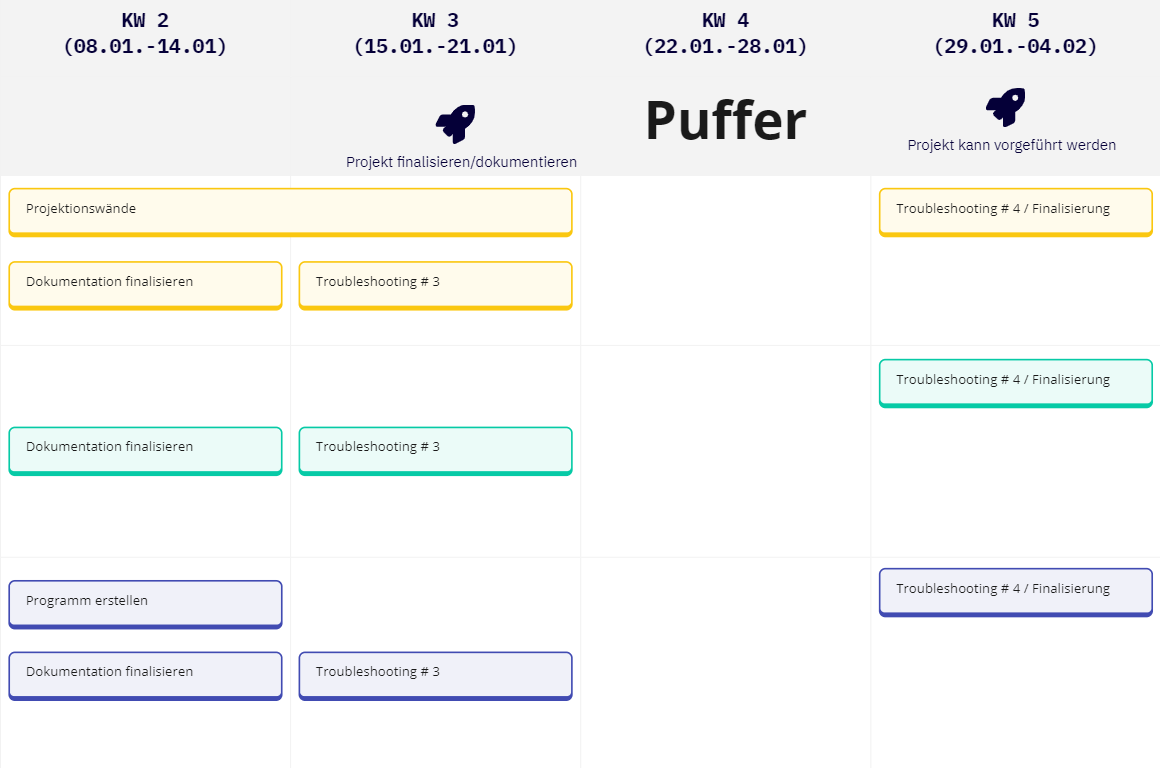
\includegraphics[scale=0.4]{road3.png}
 \captionof{figure}{Roadmap Teil 3}
\end{flushleft}

\end{document}